\documentclass{article}
\usepackage{amsmath}
\usepackage{graphicx}
\usepackage{float}
\usepackage{hyperref}
\usepackage{fancyvrb}
\usepackage{enumitem}
\usepackage{matlab-prettifier}
\setlength{\parindent}{0pt}
\graphicspath{{../images/}}

\title{CS663: Digital Image Processing - Homework 3}
\author{Harsh $\vert$ Pranav $\vert$ Swayam} 
\date{October 1, 2024}

\begin{document}

\maketitle
\section{Homework 3 - Question 1}

For both the parts of the question, we have performed filtering for parameter values 40 and 80 after doing appropriate padding. The results are shown below.

\begin{figure}[!htb]
    \centering
    \begin{minipage}[b]{0.45\textwidth}
        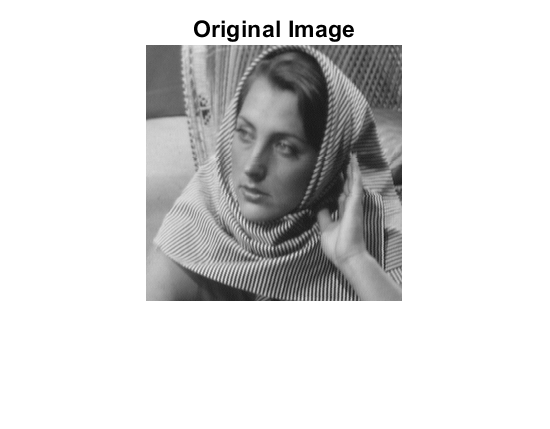
\includegraphics[width=\textwidth]{Original_Image.png}
        % \caption{Noisy \texttt{barbara256}}
    \end{minipage}
    % \hfill
    \begin{minipage}[b]{0.45\textwidth}
        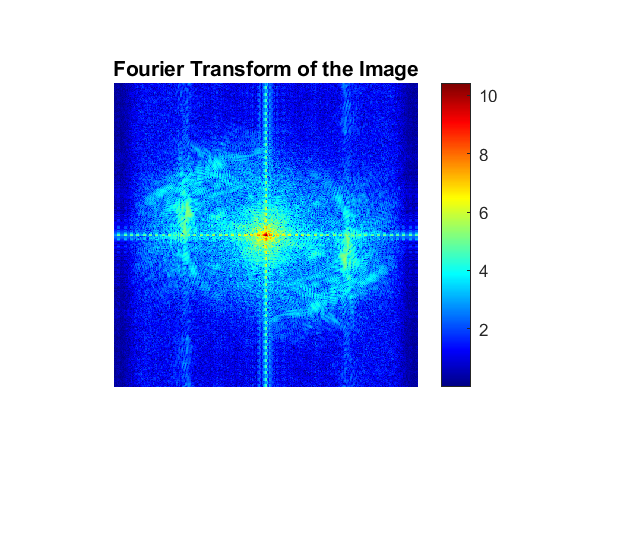
\includegraphics[width=\textwidth]{Fourier_Transform.png}
        % \caption{Noisy \texttt{kodak24}}
    \end{minipage}
\end{figure}

\vspace{-10pt}

\subsection*{(a) Ideal Low Pass Filter}

For cutoff frequency 40:

\begin{figure}[!htb]
    \centering
    \begin{minipage}[b]{0.3\textwidth}
        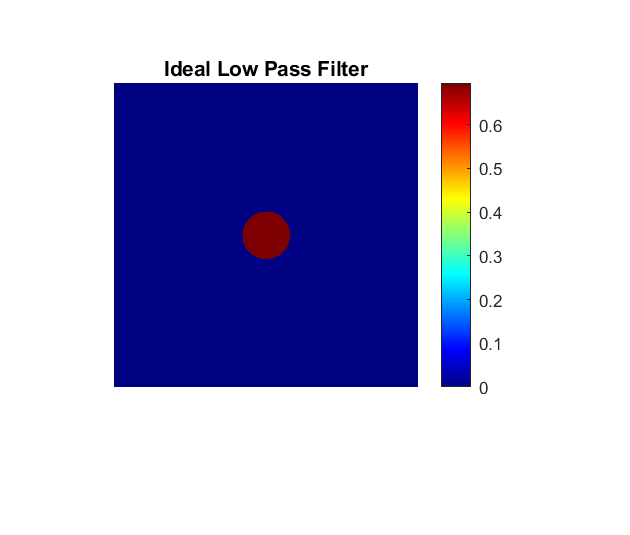
\includegraphics[width=\textwidth]{Ideal_Low_Pass_Filter.png}
        % \caption{Noisy \texttt{barbara256}}
    \end{minipage}
    % \hfill
    \begin{minipage}[b]{0.3\textwidth}
        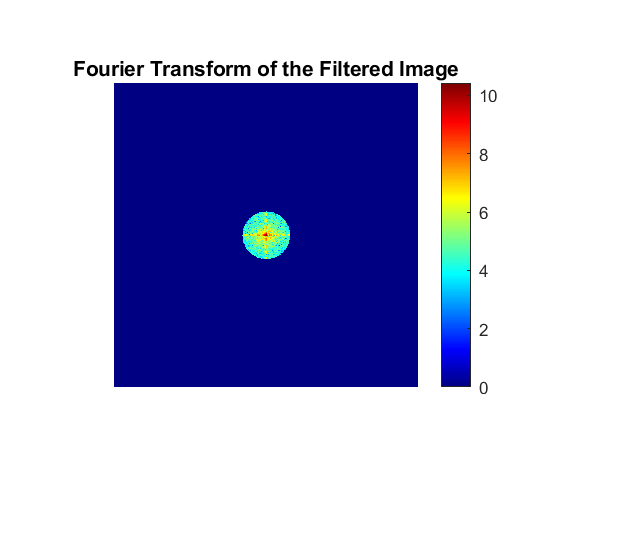
\includegraphics[width=\textwidth]{Fourier_Transform_Filtered.png}
        % \caption{Noisy \texttt{kodak24}}
    \end{minipage}
    % \hfill
    \begin{minipage}[b]{0.3\textwidth}
        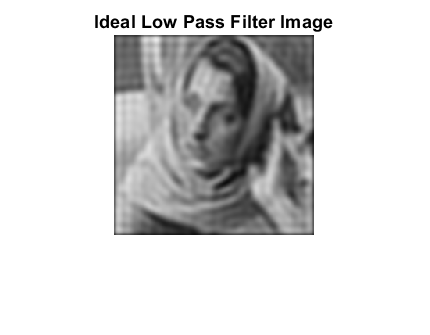
\includegraphics[width=\textwidth]{Filtered_Image.png}
        % \caption{Noisy \texttt{kodak24}}
    \end{minipage}
\end{figure}

For cutoff frequency 80:

\begin{figure}[!htb]
    \centering
    \begin{minipage}[b]{0.3\textwidth}
        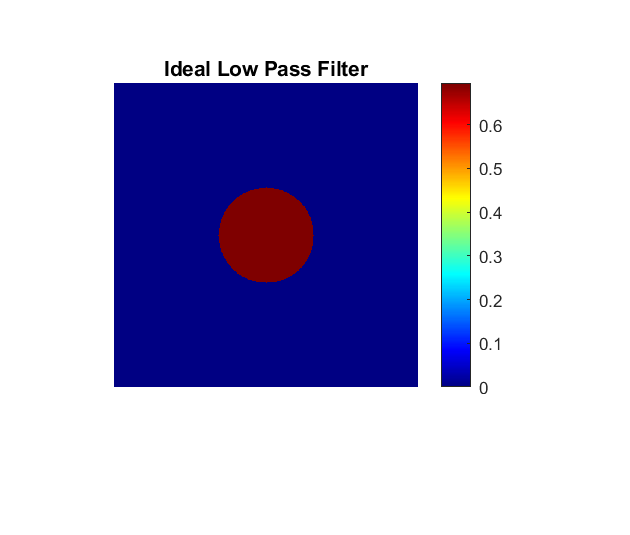
\includegraphics[width=\textwidth]{Ideal_Low_Pass_Filter_80.png}
        % \caption{Noisy \texttt{barbara256}}
    \end{minipage}
    % \hfill
    \begin{minipage}[b]{0.3\textwidth}
        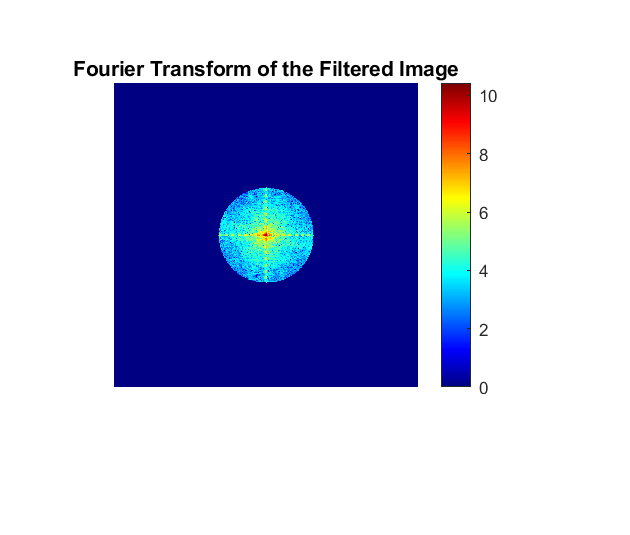
\includegraphics[width=\textwidth]{Fourier_Transform_Filtered_80.png}
        % \caption{Noisy \texttt{kodak24}}
    \end{minipage}
    % \hfill
    \begin{minipage}[b]{0.3\textwidth}
        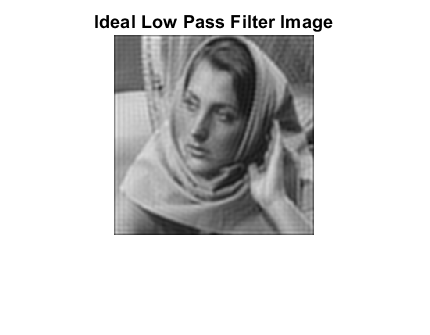
\includegraphics[width=\textwidth]{Filtered_Image_80.png}
        % \caption{Noisy \texttt{kodak24}}
    \end{minipage}
\end{figure}

\newpage
\textbf{Observations:} 
\begin{itemize}[noitemsep]
    \item As the cutoff frequency increases, it makes higher frequency components visible. This is evident from the fact that the image becomes more sharp as the cutoff frequency increases.
    \item There is a presence of ringing artifacts in the filtered image.
\end{itemize}

\subsection*{(b) Gaussian Low Pass Filter}

For $\sigma$ = 40:

\begin{figure}[!htb]
    \centering
    \begin{minipage}[b]{0.3\textwidth}
        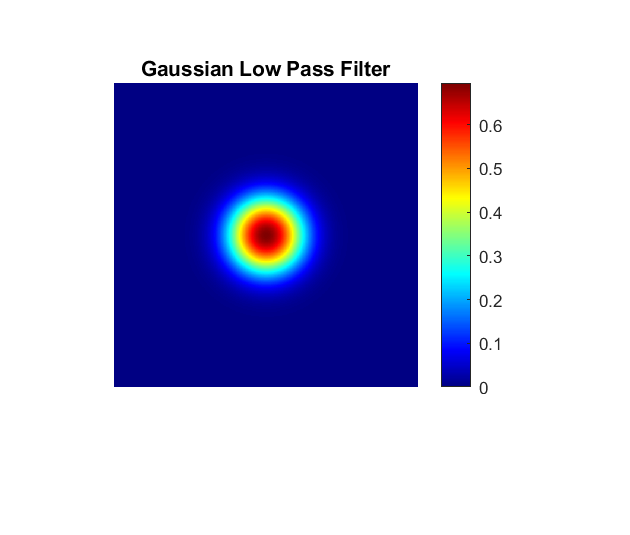
\includegraphics[width=\textwidth]{Gaussian_Low_Pass_Filter.png}
        % \caption{Noisy \texttt{barbara256}}
    \end{minipage}
    % \hfill
    \begin{minipage}[b]{0.3\textwidth}
        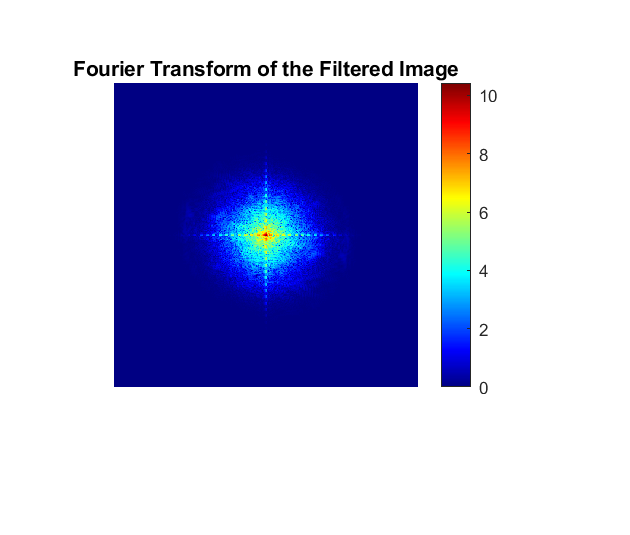
\includegraphics[width=\textwidth]{Gaussian_Fourier_Transform_Filtered.png}
        % \caption{Noisy \texttt{kodak24}}
    \end{minipage}
    % \hfill
    \begin{minipage}[b]{0.3\textwidth}
        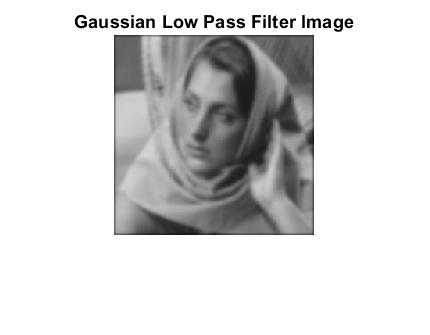
\includegraphics[width=\textwidth]{Gaussian_Filtered_Image.png}
        % \caption{Noisy \texttt{kodak24}}
    \end{minipage}
\end{figure}

For $\sigma$ = 80:

\begin{figure}[!htb]
    \centering
    \begin{minipage}[b]{0.3\textwidth}
        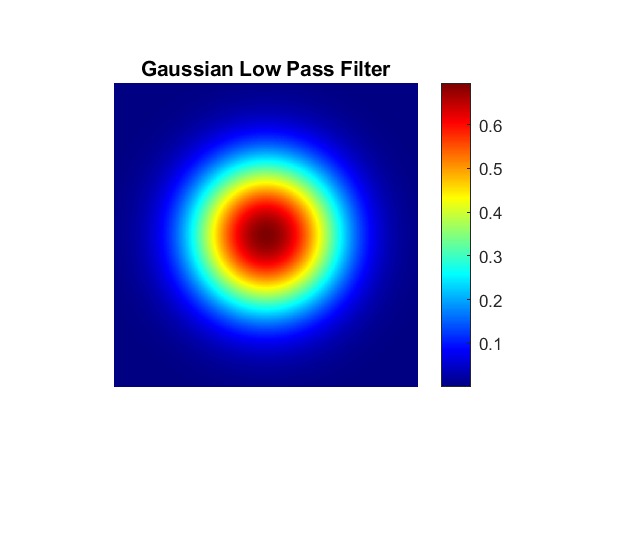
\includegraphics[width=\textwidth]{Gaussian_Low_Pass_Filter_80.png}
        % \caption{Noisy \texttt{barbara256}}
    \end{minipage}
    % \hfill
    \begin{minipage}[b]{0.3\textwidth}
        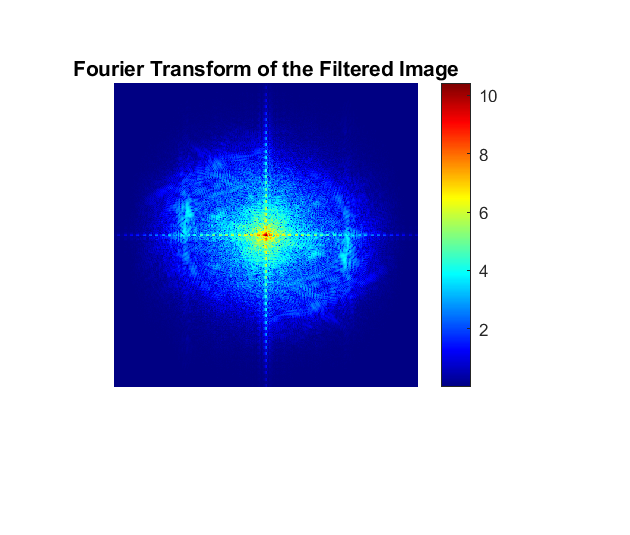
\includegraphics[width=\textwidth]{Gaussian_Fourier_Transform_Filtered_80.png}
        % \caption{Noisy \texttt{kodak24}}
    \end{minipage}
    % \hfill
    \begin{minipage}[b]{0.3\textwidth}
        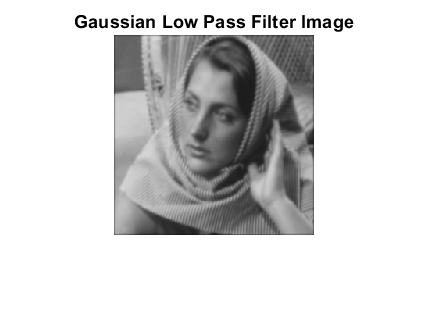
\includegraphics[width=\textwidth]{Gaussian_Filtered_Image_80.png}
        % \caption{Noisy \texttt{kodak24}}
    \end{minipage}
\end{figure}

\textbf{Observations:}
\begin{itemize}[noitemsep]
    \item As the value of $\sigma$ increases, the image becomes more sharp.
    \item The ringing artifacts are less prominent in the Gaussian filter as compared to the ideal filter.
    \item Weakening of high frequency components (contrary to elimination). Hence, the Gaussian filter is more smooth as compared to the ideal filter.
\end{itemize}

\end{document}